\chapter{Introduction}
\label{sec:Introduction}
Creating network applications nowadays might be a complicated process of design which involves long series of research and experiments or, on the other hand, it might be a fairly simple procedure that takes only a tenth of its time and effort. In both cases, the most frequent evaluation metric is the scalability of the application, more than a thousand of lines of code or the complexity of the model. With the rise in popularity, the usage of network applications increases, which in consequence results in an increase in the frequency that the application is requested to serve its functionality. This growth can be calculated and included at the planning level, thus becoming a good programming practice that places itself close to other widely approved design patterns. With no doubt is scalability starting to play a more important role, being often set at the same level with such issues like portability or security[quote]. The present thesis aims to introduce an application that by its original functionality would heave the potential to become a heavy traffic network application with numerous active users. In this chapter the reader can find an overview of popular notes taking applications, understand the basis of Version Control Systems, and learn about more technical sections regarding the Python programming language as well as terms of scalability in a Google App Engine product.

\section{Popular notes taking applications}\label{sec:popular_apps} 
No matter if the user works on a small task like plan a holiday or whether they prepare a list of ideas which they aim to share secretly with their coworkers, a computer application will be a useful help.     

Currently, users have a rich variety of notes taking applications to choose from. One group of applications represents the idea of simple user interface which mimics the well known sticky notes or cork board where the notes are not long and relatively easy to find. Flagship representatives of this group are the Sticky Notes\footnote{This notes taking application used to be the default for notes taking under GNOME, one of the highly popular Linux desktop environments.}, Knotes\footnote{This application is a component of another application called Kontact, which is frequently used with KDE Linux desktop environment.} or the Stickies\footnote{A small and handy application which comes with Apple's Mac OS X that has rivals, e.g. SketchBox aiming at the possibilities of customization.}.The above applications offer simple text highlighting, syntax correction and general layout customization. On the other hand, the remaining group of applications has more features to offer, like rich text formatting with broad fonts support and a possibility of embedding multimedia elements and hyperlinks. Moreover, a number of the applications make use of Internet accounts where notes might be edited and tagged. Because of the great diversity among the applications, it seems worth presenting two of them which appear to deserve special attention and the below sections will briefly introduce and compare both.

\subsection{Google Notebook}\label{subsec:google_notebook}
The first application that appears remarkable is Google Notebook, a Google company product\footnote{Google offer a variety of products. Right next to the browser and the Gmail e-mail service, applications like Google Calendar, Google Docs, Picassa Web or YouTube reach more and more users.} open to the end user without charge or special restrictions. It makes use of typical Google design patterns, which makes its usage naturally easy for users familiar with other Google applications. What is more, Google Notebook has a number standard elements like bookmarks and tags, which shorten the search time when notes are kept in groups. Apart from that, the interface has extended WYSIWYG\footnote{WYSIWYG is an acronym for What You See Is What You Get and is used when referring to editors having user friendly interface, operating on a markup language (i.e.. HTML or \TeX) but at the same time allowing the user for manipulation of the output without having sound command of the markup language.} functionality, which makes the rich text formatting user friendly.

For various reasons, users might like to export their notebooks. With Google Notebook this task is said to be easy and the user has three possibilities to do it: export to HTML format, print or export to Google Doc format. What might be considered as even more practical is the opportunity to collaborate on a notebook with other people by marking the notebook as shared and then inviting others to contribute to it by passing a list of emails. This functionality allows for outstanding user experience where the users may share their ideas by working on one notebook simultaneously or separately. Nevertheless, Google was required to implement a simple Version Control System (henceforth VCS) within the feature in order to merge the parts into one piece and thus handle potential conflict situations. To give an example, a conflict might occur when two ore more users are editing the same content, i.e. the same sentence, but in different ways which makes further merging impossible. The way the situation is handled by Google is presented on the below picture \dots. As a result, the user then decides which version is the correct one. The above is only one of the two possibilities that VCS offers in that case. The second one is based on prioritizing performed by the user, where the modification time is registered and the conflict situation is overwritten with the version of the highest priority. All in all, that might appear as an interesting solution, but it also seems that it may lead to mistreating others users' work without an opportunity to notice and react to the conflict.

Finally, what may seam of insignificance importance, but is of huge significance in the light of the dynamic market growth of Internet applications, Google Notebook may be relatively confident of its position. As a matter of fact, already in May 2006 had Google released the initial version of Google Web Toolkit (henceforth GWT), which allowed for huge gains of Java script and CSS compression caring for cross browser compatibility. As a consequence, nowadays GWT is a powerful tool that provides the designer with the opportunity to make the Web based interface that works as required on a majority of browsers (including mobile devices) available on the market. That may seam even more significant, as the idea of having one's own notebook on mobile devices has a great potential. 

\subsection{Evernote}\label{subsec:evernote}
The second notes taking application that is worth describing is Evernote, which is a commercial product belonging to Evernote Corporation. It has a functional interface, a bunch of unique features and a still growing group of users. Moreover, the application supports multiple mobile devices, like various operating systems, and allows for adding, modifying and grouping notes taken by its users in a swift manner. Further advantages of the application regard the approach to how the notes are made in Evernote. Specifically, the product provides the opportunity to embed various multimedia elements in the notes, which converts the note taking into a process similar to editing a blog entry. Additionally, Evernote allows for clipping all items found on the Internet, from books, through cooking recipes, to interesting articles that the user wills to return to later. To take the argument further, the latter is possible when they use Evernote on the same or another device which has the product installed. It is worth mentioning the fact that this particular feature is especially useful to users dealing with a massive amount of information that cannot be read or memorized straight away and which, thanks to Evernote, may be stored in an easily searchable way. Yet another distinguished feature of Evernote is that images added to the product are also searchable, which means that text inscribed in the pictures is recognized as any other text, a point in case being a business contact card added to Evernote in couple of seconds by taking its photo, which may be afterwards found by typing in keywords from the card. By taking a photo of a ticket, bill or any other element with text element, Evernote users find it easy to use the elastic tool for importing data to their notes that otherwise would become lost or that would need significantly more time to arrive onto the product in the traditional way.

As mentioned in the beginning of this section, Evernote is a commercial product, which means that its code is proprietary software of Evernote Corporation. It may be used without charge with certain limitations, i.e. no collaboration option, limited file synchronization formats and lower monthly rate of multimedia elements that may be clipped to the application. Not surprisingly, free users are also required to accept typical promotion and advertisement materials in order to use the application. On the other hand, the cost of a premium account with extended options and lower limitations is 5\$ a month or 45\$ for a year, which still remains a reasonable price for such an interesting tool.      
 
\subsection{Comparison}\label{subsec:vcs_comparison}
The above mentioned programs represent features with outstanding potential, yet defiantly, they fail to exploit all the features found in applications available on the market. Here, dynamics is an important factor which tends to follow the way users make use of the Internet daily, which should be considered especially when designing any kind of network application targeting an audience of considerable size. Fulfilling the requirements of keeping the speed of market changes and evolving with its users, the applications do not have their market success guaranteed, however, disrespecting the rules might generate a higher cost for the application -- losing all its users. Another rule that seems to be of significant importance is first user experience, which most commonly is built on the perception of the interface. Since currently users enjoy a wide choice of products, it is either the unique features of the application or the interface which trigger interest when users pick a product, which is easily translatable into the decision which application the user decides to use for longer and which they will never open again. Consequently, due to the fact that users naturally tend to have different habits and expectations, a rule of keeping the product as simple as possible supersedes applications with numerous advanced features and a complicated interface and it is this rule that emerges from all rankings of top rated notes taking products. Another conclusion could form a rule that the more a web application mimics the usage of tools that their users could be already used to, the more its chance for success grows. Definitely, one of such confessions for a notes taking application would be note sharing and the possibility to work on notes in smaller groups of contributors. Although a custom solution might be used for the latter, a real Version Control Systems like the one described in section~\ref{sec:popular_vcs} is used to handle various collaboration scenarios and continuously prove its helpfulness for developers working on projects of various scales. 

\section{Popular Version Control Systems}\label{sec:popular_vcs}
In order to describe VCS, the following scenario has been taken into consideration. A group of developers are working together on a piece of software. Most probably, they divide the work into functional pieces and complete the necessary planning. Afterwards, they begin to code according to their company's coding standards, the approved methodology or favorite schema. Doubtlessly, the developers are required to interact not only by exchanging ideas but also by working on the same parts of code simultaneously and it is at that point when they prefer to be uninterrupted while working on their code, by the same time allowing other developers to track their progress or to make modifications they might find necessary to complete. That basic need was the primary reason for inventing an external software which additionally could inform the developer what changes have been implemented since the last time they worked on the code, a software that merges the work of several developers. 

Although currently there exists a wide variety of VCSs offering diverse functionality, the true golden age for VCS has started relatively recently. It was in 2001 when after the remarkable success of Concurrent Version Control (henceforth CVC) Jim Blandy and Karl Fogel released a project aiming to replace CVC by fixing the renown inconveniences of the system, introducing a more appealing architecture and a cleaner code~\cite[page 11]{hg_book}. The project was called Subversion, also known as SVN by its command line utility name, and despite the fact that it is CVC that probably holds a title of the world's most widely used VCS, it is SVN whose birth resulted in dozens of new and original concepts. Some of the concepts emerged soon after SVN was released and that regards Mercurial, Bazzar and Darts; others, like Git or Guilt, required time to evolve and attract new developers. Nevertheless, the first VCSs are much older and one of the very first ones, Source Code Control System, was grounded in 1970s at Bell Labs. Taking into account the fact that at that time computer popularity was not that significant, the dynamics in which the VCS systems were developed during those days would seem remarkable. The following section will describe one of the most outstanding VCSs which will serve as a base for the application presented in the practical chapters of the thesis.

\subsection{Mercurial}\label{subsec:hg}
Mercurial is a Distributed Version Control System (henceforth DVCS) and features of the latter will facilitate the understanding of how the Mercurial system might be used and which use cases it suits well. In comparison to SVN or any other centralized VCS, where only the main machine contains the repository with its history, DVCS provides every user with access to history on their hard disk, which in consequence enables the user to exploit the repository with all the available tools. Moreover, work remains undisturbed disregarding the server status as it is the user who plays the role of a server for themselves. This simple modification to the concept of centralized VCS was exactly what dynamically expanding Open Source projects were seeking. Each developer might work on their repository allowing others to use their work by performing merge operations, at the same time using work of other developers in the very same way. With DVCS, network connection to the main server was no longer needed in order to enjoy a functional environment where developers could create, analyze and modify the code whenever they preferred to. The latter was not only a step forward in making VCS more user friendly, but also improved the performance of this system. 

The very improvement was made with the completion of a number of actions. Firstly, all repository metadata was placed on users' hard discs as there was no reason to connect to the main server in order to find, for instance, the date when modifications of a class unexpectedly stopped working correctly. Secondly, the system was made fully scalable as in the case of DVCS, central machine, if present, is only used as a public main stream version of a project consuming minimum of the machine CPU and disc space, its only role being to allow users to download the most recent version of the repository. Thirdly, by having the project with its history saved on every developer's hard disc, the problem of backups was automatically solved and ensured total crash security. All the above advantages taken into account, it must also be made clear that  maintaining the repository with its history results in a significantly larger cumulative size of it. Indeed, metadata combined with development history forms a naturally additional overhead being stored on users' discs, even if typically it does not exceeds a tripled size of a free repository. Costly as it may seem, the latter is the price DVCS users agree to pay for additional functionality which the system offers. 

It is also worth to note that the system's design has been what encourages its users to experiment. Certain operations, e.g. branching or forking, were created solely for that purpose. Moreover, it is worth to mention that making frequent tries beyond the main version was a desirable feature that was added to the system not only to maintain the cleanliness of the history, but also to allow developers perform as many tries as they are willing to, thus letting the system play a remarkable role in Open Source communities by helping to build and keep the community healthy~\cite{git_talk,svn_talk}. Finally, to bring the last, but not least advantage of Mercurial, it cannot escape attention that the DVCS has a number of additional commercial features. Bryan O'Sullivan points in~\cite[page 6]{hg_book} the following: 
\begin{itemize}
\item{Better availability and reliability for teams scattered across the globe.}
\item{Better scalability and ease of maintainance.}
\item{Greater flexibility, which might be a value for target customer.}
\end{itemize}
What is more, Mercurial is claimed to be quicker to learn and uses similar commands to the ones used in SVN or CSV, which eases the transition regardless of the operating system (the latter will be especially useful in terms of the Microsoft, Linux and Apple compatibility used in the tool presented in the following chapters). To hit the final note, Marcurial has an efficient HTTP protocol support~\cite{google_hg_git_compare} both as a client and server application, which serves as a useful feature when the work on particular repository tends to be very active within one developer group.

\subsection{Mercurial comparison with other systems}\label{subsec:dvcs_compare}
As a matter of fact, there exist a number of other DVCSs offering interesting functionality. Atomic commits, GUI\footnote{Graphical User Interface -- it eases the usage of system to users which are not used to work with command line tools.} tools, commits tagging, tracking merge operations in the history or allowing for user defined actions just before or after certain actions performed on repository are only few of the commonly used features in DVCS comparisons~\cite{wiki_dvcs_compare}. 

With time, the already long list~\cite{wiki_dvcs_list} will probably continue to expand; nevertheless, currently the most popular alternatives for Mercurial are Git and Bazzar, the former stemming from the Linux kernel developers community and the latter being associated in close vicinity to GNU\footnote{The name “GNU” is a recursive acronym for “GNU's Not Unix!”. The GNU Project was launched in 1984 to develop a complete Unix-like operating system with free software and at the time being, it is recognizable for the GNU/Linux operating system.} developers group. The similarities between the two systems are that both are remarkable, though using slightly different concepts, and both are based on the C language, which should positively impact their performance. However, it must be stated that the language requires compilation and in consequence it might not be suitable to systems which forbid running binary programs. Another significant difference regards the level of complexity. On the one hand, Git provides numerous commands and arguments allowing for full control over the repository and its history, while on the other hand Bazzar's flagship feature is the minimum time the user must spend on learning the proper usage of the VCS, which, at the same time, makes the system similar to Mercurial. The final difference regards the repository maintenance, in which Mercurial is claimed to be most efficient, not requiring additional operations like running \texttt{git-gc}\footnote{In order to achieve a better performance of disc space utilization, users of Git are advised to run the command on a regular basis, which is often compared to housekeeping by removing unnecessary objects or performing repository objects repack and compression. Interestingly, the name \texttt{git-gc} refers to a garbage collector, or a mechanism used in various programming languages for memory control.} in the case of Git or using less disc space than Bazzar finds necessary for the same repository. 

Apparently, all three systems have reached the level of maturity, which may be concluded taking into consideration the criteria of advanced commands usage and the availability of user interface tools. However, the most important reason why developer distinguish between existing VCSs is associated with the frequently offered functionality of a particular system and the habits the user used to have. Viewing this argument from a practical perspective, it must be noted that the criteria did not serve their purpose in the case of the application proposed in this thesis. The reason why Mercurial has been chosen is that the application required a lightweight yet powerful Python-based system with good support for running over HTTP requests. Further chapters will present the features in more detail, for now suffice it to mention that the support of Mercurial would not have been equally effective if it had not been compliant with the requirements of Python, which will be explored below.

\section{Role of programming language}\label{sec:languages}
Currently there exist dozens of programming languages among which some were invented years ago and still continue to evolve and the other, represented by newer ones that join most recognized elements of their predecessors and introduce new directions for development. Disregarding the languages' history and unique characteristics, each of them may be considered as a different tool in a programmer's toolbox. Following the remark made by Cal Henderson, "scalability isn't about using any particular technology at all"~\cite[page 203]{build_scalable}; it is the engineer, his experience and his ideas which count most and the rest is merely the workshop. Admittedly, it is of utmost importance to select the right tool for right task, yet usually the most powerful gear available is not a prerequisite. Quite the opposite, some languages may perfectly play their role due to their available components used in similar projects; alternatively, they may provide the shortest way to solve the particular problem. The decision on the language is made once, as rewriting entire projects from one language to another occurs relatively seldom as the process involves redesigning certain elements, which most surely consumes a lot of effort and time. On the other hand, reaching the right decision may bring ready-made solutions for most problems arising while a project is being developed. Finally, while it is likely the user will reach developers ready to help with problems they know from experience and happy to share their knowledge, identifying the right technology, hence the most useful language, is one of the very valuable skills that come with experience build on the method of trail and error. 

The following section will introduce Python, a language that is fundamental for the subject of the thesis, with an attempt to present its role not only in the tool itself, but also in the current programming language environment.
  
\subsection{Python}\label{subsec:py}
Python is a general-purpose programming language~\cite[page 3]{py_nutshell} and the variety of fields in which it has proved to be useful may impress. A shortened list of purposes the language served, according to Matt Telles~\cite[page 13]{py_power} includes:
\begin{itemize}
\item{Cinematography}
\item{Business information}
\item{Aviation}
\item{Government}
\item{Chemistry}
\item{Weather}
\item{GIS}
\item{Engineering}
\end{itemize}
The list may also be completed with universities, where Python is frequently used, with numerous lecturers following the reasoning of prof. James A. Hendler: "I have the students learn Python in our undergraduate and graduate Semantic Web courses. Why? Because basically there's nothing else with the flexibility and as many web libraries"~\cite{py_quote}. The reason why the language has gained such popularity through years may be best explained by its history.

Having been developed in the 1990's by a Dutch programmer Guido van Rossum, Python grew in popularity in an exceptionally dynamic manner since 2000~\cite{py_code_swarm}. Throughout the evolution, the language has had a number of functions developed, which nowadays tend to be presented as the key features distinguishing Python from other languages ~\cite{py_about}:
\begin{itemize}
\item{Very clear, readable syntax}
\item{Intuitive object orientation}
\item{Full modularity, supporting hierarchical packages}
\item{Very high level dynamic data types}
\item{Extensive standard libraries and third party modules for virtually every task}
\item{Extensions and modules easily written in C, C++ (or Java for Jython, or .NET languages for IronPython)}
\end{itemize}
Beside the above, it is important to note that Python belongs to a group of interpreted languages, which means that the code might be transformed to a hardware-independent byte-code and then used by the interpreter to call machine statements. To compare the latter with the classic cases, typically compiled language code is transformed to hardware-dependent machine commands and loses flexibility, having to combine with every platform the language is supposed to run on after the tiniest source code modification. This is easily avoidable in the case of Python as the cross-platform code is flexible enough to debug and maintain. 

Moreover, it should not escape attention that Python is written in C, using the language in a highly optimized way while running functions. Consequently, the code may stay both compressed and fast, which makes the source code files shorter and more user-friendly in terms of their readability. That is another reason, next to wide documentation on why "Python is friendly... and easy to learn"~\cite{py_about}. Finally, what is not negligible is the licensing issue. The fact that Python is distributed under an Open Source license makes the language freely usable and distributable not only for non-profit use, but also for commercial purposes without additional restrictions. The latter might have yet broader meaning as in the light of law, Python cannot become a closed and commercial product, which leaves developers relying on their creativity stemming from nothing else than the use of the code. This particular feature is one of the characteristics distinguishing Python from other languages and the below section will present other points of comparison.

\subsection{Comparison with other languages}\label{subsec:lang_compare}
It is fairly difficult to objectively make general comparisons on programming languages and as it has been mentioned in \ref{sec:languages}, languages may be compared on the basis of the different tools they offer to programmers in order to solve particular problems. Since the case also regards experience and cooperation with already available tools, it is evident that pointing one language as the optimum choice for solving all possible problems, even regarding a single application, is impossible, which is a reason why software projects used to be written by use of more than one language. Nevertheless, it might be interesting to present the graphical illustration of community activity of particular languages. For this purpose, C\#, C++, Java, Python and Ruby have been chosen as the most popular object-oriented programing\footnote{Object Oriented Programming OOP is one of programing paradigms that operates on data structures called objects. With such operations like inheritance, data abstraction or encapsulation it allows for effective attempting complicated problems in a human friendly way.} languages. The graphs below differentiate the activity of these languages in two perspectives: by the number of projects as well as by the number of active contributors.
\begin{figure}[ht]
  \begin{center}
    \subfigure[\textbf{Monthly Projects}.~\cite{ohloh_projects} \newline The lines show the count of projects with at least \newline one line of code changed in a month.]{\label{ohloh_projects}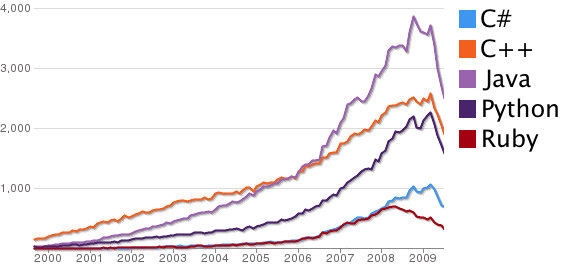
\includegraphics[scale=0.36]{img/Monthly_projects.png}}
    \subfigure[\textbf{Monthly Contributors}.~\cite{ohloh_contributors} \newline The lines show the number of developers who have contributed at least one line of code in each month]{\label{ohloh_contributors}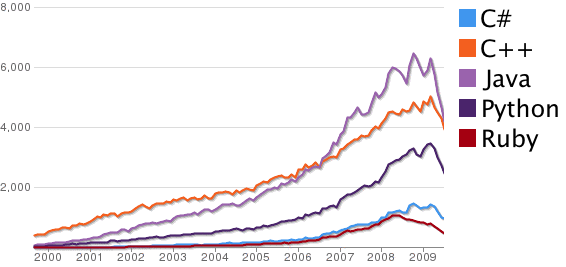
\includegraphics[scale=0.36]{img/Monthly_contributors.png}}
  \end{center}
  \caption{Programming languages activity graphs.}
  \label{fig:ohloh_lang_graph}
\end{figure}
The obvious conclusion that may be drawn from the graph on figure~\ref{fig:ohloh_lang_graph} is that the Python community remains active, maintaining its position among the top active languages for a significant amount of time. Despite the passing years, Python keeps pace with changes in the software world and seems to be an interesting option with proven usability in miscellaneous areas. No matter if the application is supposed to perform a single job once or scale-wide, being deployed on various machines, Python offers ready-to-be-used tools.
 
\section{Scalability}\label{sec:scalability}
In order to define the term scalability, the work of Cal Henderson will be cited~\cite[pages 203--204]{build_scalable}, where he points three characteristics that scalable system should have:
\begin{itemize}
\item{The system can accommodate increased usage.}
\item{The system can accommodate increased dataset.}
\item{The system is maintainable.}
\end{itemize}
The definition does not seem to require much additional explanations; however, it provides only the basic criteria which should help to understand the meaning of the term, at the same time failing to exploit the problematics standing behind it. It may be crucial to understand that scalability as a process of planning ought to be grounded before the increase happens. To take the argument further, scalability pattern could signify an 'increase ready' one, which in the real-world project has certain consequences:
\begin{itemize}
\item{Capital investment will be made.}
\item{The system will become more complex.}
\item{Maintenance costs will increase.}
\item{Time will be required to act.}
\end{itemize}
Accordingly to the author of  "Scalable Internet Architectures"~\cite[page 8]{scalable_arch}, the above four points are guaranteed when scaling any system. Therefore, scalability has its own cost, one making the desired growth on scale more profitable if not only possible. While horizontal scaling means expenses for an extra number of elements that a brand or model that has already in use, vertical scaling would aim in replacing existing components with more powerful ones. At the same time both of them, according to their concept, assume minimum required work on architecture, even if horizontal scaling is regarded as the only 'true'~\cite[page 5]{scalable_arch} type of scalability. 

Vertical scaling has two disadvantages when related to the horizontal scaling model. The first drawback are the limitations above which a system using vertical scaling fails to scale more. The issue stems from hardware limitations as system components can only be exchanged to more powerful ones up to a certain limit dictated by the current technology level. Secondly, cost efficiency appears to be a n obstacle as the vertical scaling cost model does not scale linearly~\cite[page 204]{build_scalable}. Investing more in medium class components seams to be more flexible and financially effective to make the system scale wider. On the other hand, it is remarkable that the system becomes more complexed as adding numerous components increases the risk of failure of a single element of system. This consideration should also take into account that horizontal scaling concept utilizes already known and well proven components, whereas vertical scaling requires from the engineers additional work to learn and check elements installed.

To conclude the above argumentation, it becomes obvious that scalable applications bear a cost which allows their developers feel confident in case the system will gaining popularity. By choosing horizontal scaling model, the system and the expanses remain under control, which also leaves the system reliable to its users now enjoying it with a guaranteed level of quality. 

When developing a web based application, the role of developer is not only limited to writing the code, especially if more users are interested to try their application. Depending of the application, specific features will be needed, including a third-party software that needs to be installed and configured to let the application serve its purpose, which cannot be negligible as it consumes considerable amount of time and has impact on the application when the level of usage increases rapidly. A product called Google App Engine, introduced in the next section, has challenged that process.  
 
\section{Google App Engine platform}\label{sec:gae_general}
Google App Engine (henceforth GAE) is one of the Google products that provides web applications with hosting, data storage and remarkable performance networking by using rock-solid Google infrastructure~\cite[page 1]{gae_develop}. It was primary supporting only Python runtime, but starting from April 2009 it has also been made available for Java runtime. This product is continuously developed by the Google team and newer versions of Software Development Kit SDK become regularly released. GAE is an interesting initiative enabling developers to use Google's own infrastructure like GFS\footnote{GFS is an acronym for Google File System. It is an internal technology of Google that allowed to build distributed, vault tolerant jet hight availability system for various of Google services.} or BigTable\footnote{BigTable is Google concept for Data Store. It is a kind of hash table database with many advanced features like entity groups or transactions. As claimed in the official BigTable paper~\cite{bigtable_about} many of Google projects including Google Earth and Google Finance use BigTable entities to store their data.}. The main idea behind GAE was to let developers concentrate on developing their application and make the Google team care for the infrastructure, which according to the GAE homepage~\cite{gae_homepage} may be accomplished easily. Google points~\cite{gae_why} a few reasons why App Engine might be the right choice: 
\begin{itemize}
\item{Easy to get Started. Users of GAE do not worry about system administration, tweaking the configuration, buying extra machines of search for another static content server.}
\item{Automatic scalability. By organizing the code to fit the GAE design, the application becomes well structured and easier to scale when running on Google infrastructure.} 
\item{The reliability, performance and security of Google's infrastructure. Taking advantage of the 10 years of experience in building performance driven and secure systems, Google applies the same rules for applications hosted on GAE just like their own applications.}
\item{Cost efficient hosting. When running on GAE, machine resources are not an issue anymore -- in case an application requires more power, Google offers a competitive pricing policy. First of all, the billing application built into GAE enables the user to monitor their resources and make changes to the plan in real time. Secondly, protection against running out of resources by one high peak of traffic make the conditions set by Google not only interesting from the technical point of view, but also highly business competitive. Additional calculations can be found in section~\ref{}}
\item{Risk free trial period. After creating an account and publishing an application people can straight away start to use it with a generous limit of about 5 million page views a month, which is free and without any commercial obligations.}
\end{itemize}

Apart from the Google massive infrastructure, GAE can not be compared to any of the LAMP\footnote{Primary and most popular acronym is LAMP and it stands for Linux, Apache, Mysql, and PHP that on other operating systems this became WAMP for Microsoft Windows and MAMP in case of Apple's Mac OS X. This is the basic infrastructure needed to run web based applications.} packages. It extends that idea for a locally developed environment as well as a 'production' environment, where the application runs after deployment. With the SDK provided by Google for the Mac OS X, developers can make use of the GoogleAppEngineLauncher, which eases the development process and as a result, provides the possibility of uploading the developed application to Google with one click on a button. This very application is presented on figure \ref{gae_launcher}.
\begin{figure}[h]
\begin{center}
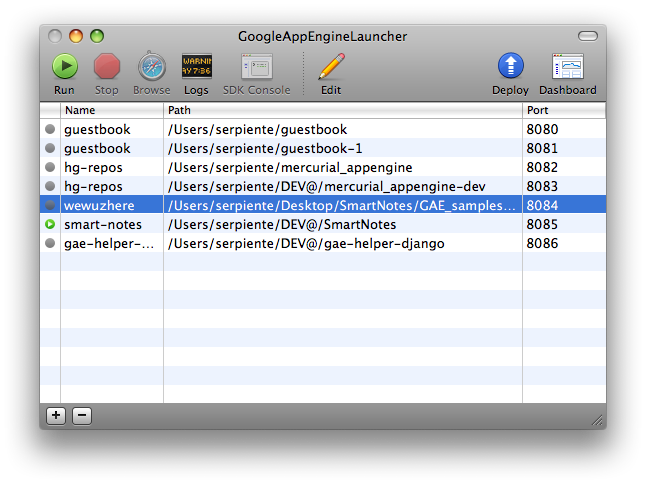
\includegraphics[scale=0.4]{img/gae_launcher.png}
\caption{Goole App Engine launcher application.}
\label{gae_launcher}
\end{center}
\end{figure}

Another set of features which are often found useful in the application development process or which extend the basic GAE functionality for even better performance and flexibility are:
\begin{itemize}
\item{Application dashboard. The tool is the developer's fundamental help in navigating other tools and creating application status overview with figures like used resources, recent load, recent errors generated by the application and charts showing the number of requests per second or milliseconds per request, to name a few. The dashboard binds together all GAE components.}
\item{System status. The service provides the status of the GAE system itself. Google has massive resources and makes use of redundancy, however, for various reasons, it seems reasonable to have the GAE system monitored as well. The tool provides information on when significant maintenance job is planned as well as certain pieces of data on component status and the latency of write or read operations. Moreover, the service is available as an alert RSS feed in order to keep developers updated on the recent changes without the need to continuously following the web page.}
\item{Memcashed. The technology was invented by the developers of Danga Interactive, a company acquired by Six Apart. Its creators realized they may achieve a remarkable gain on performance by storing functions output in memory and in case of subsequent calls to that functions, by returning the stored value, making use of the invariance of the returned values. In the opposite case, the stored (cashed) values are removed form Memcashed and replaced with the new value. Another advantage of the technology is its transparent distribution among numerous machines.} 
\item{Interactive console.The facility allows for interacting with the application both on the local and the 'production' side. By the use of it, developers may complete control tasks, interact the datastore or perform higher level debugging.}
\item{Datastore}. It is one of the main elements of GAE and since creating files is not permitted in the latter, datastore fulfills the role of a base storage system. What might be impressive about the system is that it is a schema-less\footnote{It brakes the SQL methodology where entities are defined in the code of application and can be changed and moved around just by a few lines of code changes.} distributed storage system. By being built on the top of BigTable, it has the same scalable characteristics and provides a friendly API for data modeling and performing queries. 
\item{Datastore data browser. Owing to the browser, the storage engine can be browsed in a user friendly way, providing data that is clearly organized, by the same time allowing to perform basic CRUD\footnote{CRUD is an acronym for Create Read Update and Delete. This is a group of basic operations that are most frequently performed on data sets.} operations. The browser may be compared to the graphical SQL administration tools\footnote{The most popular are the phpMyAdmin in case of MySQL databases or pgAdmin in case of PostgreSQL databases.} .}
\item{Cron jobs.} As a matter of fact, Cron is not an invention of Google; it is an older idea stemming from the UNIX world, with the basic role defined as running user-defined tasks synchronously. The GAE Cron exploit the role completely, providing a configuration file that defines what and when should be actioned. An example of its usage might be sending weekly reports to registered users summing up market behavior in the case of a business analytics application.     
\item{Task queues.} The feature extends the Cron jobs functionality, allowing the developer to create a queue with parameters like number of tasks to run per second, and then append tasks to that queue, which amounts to an efficient way of run asynchronously a number of jobs in the background when the system load is lower.  
\item{URLfetch service. The service allows to perform HTTP and HTTPS requests and therefore to interact with other applications.}
\item{Mail service. With the help of the service, the application can send mail messages without the need to set up a SNMP server.}
\item{Images service. The service offers images manipulation operations like resizing; also, changing the brightening and contrast can be easily done.	}
\item{User service. Users may log in to the service with their Google account and the functionality is usually effectively used for saving user settings and the identification.} 
\end{itemize}
The way that some of those components fit in the Google App Engine is presented on the diagram in figure~\ref{fig:gae_request_cycle}, which gives an overview of how the HTTP request is being handled by GAE.\newpage 
\begin{figure}[h]
\begin{center}
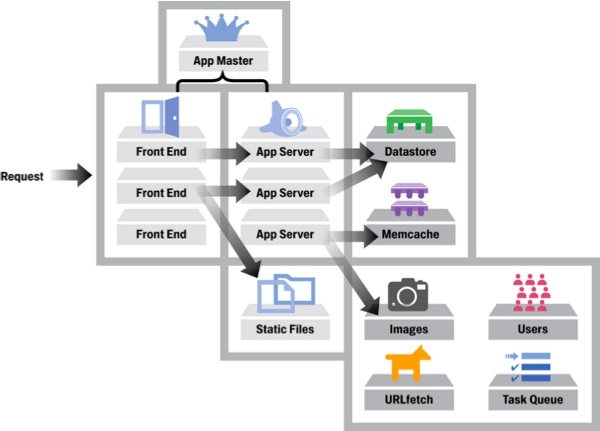
\includegraphics[scale=0.4]{img/gae_request.png}
\caption{The HTTP request life-cycle with Goole App Engine~\cite{gae_request_cycle}.}
\label{fig:gae_request_cycle}
\end{center}
\end{figure}

Finally, GAE may flaunt its developers community built by GAE users as well as Google developers working on GAE itself. Thanks to them, GAE has a detailed and clear documentation with a considerable base of practical examples. For instance, users of IRC\footnote{IRC stands for Internet Relay Chat and by use of that protocol, users can perform online conversations with a wide audience or with chosen persons.} might answer their questions by visiting the \#appengine channel on the freenode network. Besides, Google effectively promotes GAE by presenting applications developed with the help of it, which results in a rich library of resources available for beginners and advanced users willing to learn new functionality.

The following section will present the reasons of supporting GAE by Python. 
  
  
\subsection{The Python Runtime}\label{subsec:gae_py}
As a matter of fact, it was the Python language that was primarily supported by GAE. Since a number of internal Google tools were developed with the help of Python, it should not seem surprising that the first GAE runtime language has been decided to be Python, the choice having been sealed with the fact that the creator of the language, earlier employed by Google, was involved in the project.

Disregarding the implementation, the very basic role of GAE was to serve an interface for writing web applications. Therefore, the most basic usage example was to serve the HTTP requests with a code called Handlers. Apparently, it also offers a set of ready-to-use components, some of which having been introduced in~\ref{sec:gae_general}. 

Admittedly, the developer is required to decide which framework suits the needs of the tool they are creating. GAE equips them with the webapp and Django frameworks discussed in more detail in respectively~\ref{subsec:webapp} and~\ref{subsec:django}. Although the application may be extended by increasing the complication level, the developer begins with a literally empty folder and only after installing the GAE SDK does the new project template contain the following three files:
\begin{itemize}
\item{app.yaml} -- main configuration file in the YAML\footnote{YAML is an  acronym for YAML Ain't Markup Language. YAML is a data serialization format whose most remarkable advantages are its readability and optimal performance. Its alternative is JSON, which has a slightly less readable form, but on the other hand has proven even better performance in the serialization process.} format. This file enables the first line mapping of the URLs to the handlers or static files. It also allows to determine which parts require administrator privileges or which should operate over the HTTPS\footnote{HTTPS is extension of HTTP by adding cryptographic data protection. It uses the concept of asymmetric cryptography together with certificates for data protection and Certificate Authorities CA for certificates validation.}. By the use of this file, the developer may decide which files or folders should be skipped when uploading the application to Google or set the cache expiration time period for static content.   
\item{index.yaml} -- file containing the definitions of datastore indices. Its content is generated automatically and is based on the frequency and latency of datastore queries. The file may be tuned by the developer, but in most cases the default indices are sufficient to maintain the file in its basic shape.    
\item{main.py} -- bootstrap for the application. Depending on the framework used, its role may slightly differ, but it is a pure Python script that joins together the framework interface with GAE.  
\end{itemize}
The above compilation of files seems to be the optimum solution comprising the most of GAE infrastructure and leaving the developer with an opportunity to make their own decisions on which components are necessary to build their application.

\subsection{The webapp framework}\label{subsec:webapp}
Presenting any kind of web framework appears problematic as the frameworks mostly differ in details and only in few core features. For that reason, in order to describe the webapp framework without repeating its documentation, webapp framework will be demonstrated by building a simple application. It will be a demo application that exploits GAE datastore to store the user's input and present the latest three inputs in chronologically. As the purpose of this example is to focus on the framework and hold the example simple, the application-specific logic will be minimized.

It is important to mention that webapp, as a modern framework, does respect the Model View Controller (henceforth MVC) methodology, which makes the application code well organized and easier to maintain. The demo application project structure has been extended with one static HTML file and the code has been placed in the main.py file. The most significant part has been completed by adding two classes presented on the listing~\ref{code:webapp_sample}. The first, called Logs, represents the default datastore class \texttt{db.Model} and forms a MVC model. It is used for saving and retrieving data from the datastore. The second Class, named MainHandler, represents the view from the MVC and it is the true code that is run in response to user requests. Here, the class has two methods defined: one method retrieves three most recent entries from the Logs model and passes them to render a template that is then returned to the user browser; another method is initialized with HTTP POST requested from the user and after storing typed data, it redirects to the default action, or the first method. The process allows to see most recently created entry in the top position. The role of controller is distributed between the app.yaml file and then the main.py file. In case none of the regular expressions defined in the app.yaml file matches the requested URL, the main.py is evaluated and when creating an application object, the developer has another chance to define which handlers are responsible for which URLs. In this case, the \texttt{/} got assigned to \texttt{MainHandler} by calling \texttt{webapp.WSGIApplication([('/', MainHandler])}.
 
\lstset{language=Python,caption=Python classes used with webapp framework to build the demo application.,label=code:webapp_sample,
basicstyle=\scriptsize,         % the size of the fonts that are used for the code
showspaces=false,               % show spaces adding particular underscores
showstringspaces=false,         % underline spaces within strings
showtabs=false,                 % show tabs within strings adding particular underscores
tabsize=2,	                % sets default tabsize to 2 spaces
captionpos=b,                   % sets the caption-position to bottom
breaklines=true,                % sets automatic line breaking
breakatwhitespace=false,        % sets if automatic breaks should only happen at whitespace
escapeinside={\%*}{*)}          % if you want to add a comment within your code
}
\lstinputlisting{src/samples/webapp/main_s.py}

At this point, it appears worth presenting the idea of templates as it has become a commonly used technique that allows to avoid repeating work and is especially popular in web applications\footnote{Perl programmers use Template Toolkit or Mason, Ruby has its Ruby on Rails framework with templates, whereas Python has a few temple engines, with the most popular being Django templates system, Jinja 2 and Genshi.}. GAE uses the Django template system, which has clear syntax and cares for keeping the template logic and the logic-separated view. Although certain template engines use different syntax and have various tools used from template inside, the concept remains unchanged. By the help of some functions and special placeholders, templates allow for placing data into text files. The demo application presented in the thesis uses a part of template from the listing~\ref{code:template_sample}. 

\lstset{caption=Django template system example from the demo application.,label=code:template_sample}
\lstinputlisting{src/samples/webapp/template_sample.html}
Altogether, the above allowed to achieve the final result as presented on figure~\ref{fig:webapp_sample}
\begin{figure}[ht]
\begin{center}
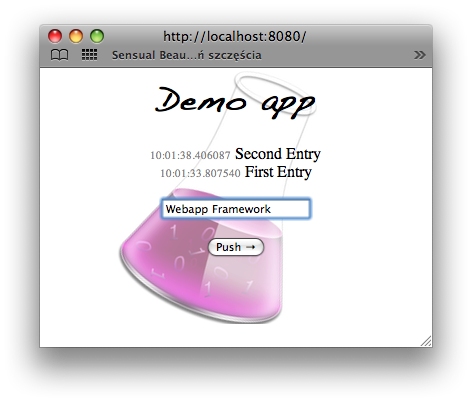
\includegraphics[scale=0.6]{img/webapp_sample.png}
\caption{Demo application done with the webapp framework.}
\label{fig:webapp_sample}
\end{center}
\end{figure}
The above is a demo application performing a simple job and the latter may be changed by adding more application logic, serving more URLs and supporting different browsers and operating systems. In this case, the complication level would certainly increase; also, most probably, the datastore model would likewise gain complexity, which is a natural process. What remains necessary to be said, even most varied applications have some parts in common, parts that are frequently used no matter what functionality is offered by the applications, an example being searching, RSS, internationalization, chronological listings and many others. In the case of a webapp framework, the points would be most probably written from the beginning. The problem has been noticed by developers of the Django framework, where the aim has been to make the code as much reusable as possible. Django supports those kinds of elements as parts of the framework or easy-to-install plugins. All in all, webapp seems to be a useful framework which has optimal performance, having low Python overhead. The solution appears to be a great choice for applications that do not need many elements  and stay focused on their basic functionality. 

\subsection{The Django framework}\label{subsec:django}
The Django web framework presentation in the fallowing section will be done by following the example application discussed in section~\ref{subsec:webapp}. The final result will be similar, yet the implementation should allow to discover some of the Django-specific features and differences between the application and the webapp framework. 

The first part in the process remains for the developer to decide which version of Django they are willing to use. If the version is one of 0.96.1 or 1.0, it becomes easer as the version can be used as a part of GAE SDK; otherwise, they are required to upload another versions as parts of the application. Secondly, in order to run Django on Google App Engine, there must be chosen a project\footnote{Currently there exist two main projects, called Google App Engine Helper for Django and App Engine Patch. The former derives from the Google team and is the officially suggested one; the latter is more popular as it supports interesting features.} that will provide all missing parts, joining the interfaces between GAE and the Django framework. Depending on the choice, project structure may be slightly different. As a matter of fact, the official Google team project seems to be more orderly and adds the following files to the structure:
\begin{itemize}
\item{appengine\_django directory -- it fulfills the role of container for all modules needed to port the Django framework to the Google App Engine platform.}
\item{manage.py -- the script allows to perform administrative tasks like removing expired sessions or all data from the datastore. It supports a set of seventeen subcommands that are helpful in the development process.}
\item{urls.py -- the file represents a controller from the MVC methodology. Its role is to support mapping the URLs to the views of MVC.}
\item{settings.py -- the main configuration file using Python setting notation. Here, additional plugins are installed and configured, as well as middleware and debugging options that might be changed.}
\end{itemize}
The last three elements \texttt{manage.py}, \texttt{urls.py} and \texttt{settings.py} are usually well known to developers familiar with the Django framework. The files are created with new projects when calling the \texttt{django\_admin.py startproject} command. The application code is organized in modules which are created by calling \texttt{manage.py startapp}. This command creates three files: \texttt{views.py}, \texttt{models.py} and the empty \texttt{\_\_init\_\_.py}, marking the newly created directory as a Python module. Specifically, the first two are placed to show model classes and view functions. Moreover, while the model class could be copied without modifications to the \texttt{models.py} file, the \texttt{MainHandler} class from the listing~\ref{code:webapp_sample} used in webapp framework needed to be split into two functions presented in the listing~\ref{code:django_views}.
\lstset{language=Python,caption=Python views functions of Django framework used to build the demo application.,label=code:django_views,
basicstyle=\scriptsize,         % the size of the fonts that are used for the code
showspaces=false,               % show spaces adding particular underscores
showstringspaces=false,         % underline spaces within strings
showtabs=false,                 % show tabs within strings adding particular underscores
tabsize=2,	                % sets default tabsize to 2 spaces
captionpos=b,                   % sets the caption-position to bottom
breaklines=true,                % sets automatic line breaking
breakatwhitespace=false,        % sets if automatic breaks should only happen at whitespace
escapeinside={\%*}{*)}          % if you want to add a comment within your code
}
\lstinputlisting{src/samples/django/views_s.py}
The main difference is the object type that is being used by the view functions: in the case of webapp, it was \texttt{webapp.RequestHandler} class and in the case of Django framework, it was either \texttt{HttpRequest} or \texttt{HttpResponse} class, which have a longer list of class methods. The webapp had a philosophy of assigning view functions \texttt{get} and \texttt{post} their corresponding HTTP methods. Django is more flexible here, allowing to use custom names and make bindings in the \texttt{urls.py} file. The second clear difference are the new functions \texttt{render\_to\_response} and \linebreak \texttt{ResponseRedirect} that are Django equivalents of \texttt{template.render} and \texttt{redirect} in the webapp framework. Finally, the HTML template file  was placed in templates directory and since the webapp uses the Django template system in this case, the only change that was require in the template was to change the default action of the HTML form to point to the \texttt{/store} method.

Summing up, the Django project has a far more complex structure. In the simple demo application files needed to change their location and the view functions needed a few modifications and when the application becomes extended with new functionality, the structure offered by Django helps tremendously in keeping the project well maintained. Besides, as mentioned in section~\ref{subsec:webapp}, Django supports elements that enable writing a reusable code, whose elements are often strongly optimized and used in the application by configuring them in a single file called \texttt{settings.py}. Finally, as it is Django that supports impressive functionality out of the box, that has great performance and that can run outside the Google App Engine, the project has a large group of developers continuously improving it, which in consequence transforms writing an application into an easier process and more fun. 